\documentclass{article}
\usepackage[utf8]{inputenc}
\usepackage[T1]{fontenc}
\usepackage[dutch]{babel}
\usepackage[square,sort,comma,numbers]{natbib}
\usepackage[hyphens]{url}
\usepackage{hyperref}
\setlength
{\parindent}
{0pt}
\setlength
{\parskip}
{1.5ex plus 0.5ex minus 0.2ex}
\usepackage[margin=3.5cm]{geometry}


\title{Gegevensstructuren en Algoritmen: Practicum 3}
\author{Robbe Degr\`eve, r0662454}
\date{13 mei 2017}

\usepackage{natbib}
\usepackage{graphicx}

\begin{document}

\maketitle
\newpage

\section*{Inleiding}

\newpage
\section{Afbeeldingen als een graaf}
Gegeven zijn onderstaande afbeeldingen met hun RGB-waarden.

\begin{tabular}{| c | c | c | c | c | c | c |}
\cline{1-3} \cline{5-7}
 (7,0,0) & (0,1,0) & (0,0,1) &  & (0,0,0) & (0,0,0) & (0,0,0)\\
  \cline{1-3} \cline{5-7}
 (2,0,0) & (0,8,0) & (0,0,5) &  & (0,0,0) & (0,0,0) & (0,0,0)\\
  \cline{1-3} \cline{5-7}
  (1,0,0) & (0,1,0) & (0,0,8 )&  & (0,0,0) & (0,0,0) & (0,0,0) \\
  \cline{1-3} \cline{5-7}
\end{tabular}

We geven iedere pixel van de resulterende afbeelding een naam om de grafe te verduidelijken. Deze namen en de \textit{pixeldistance} tussen de twee afbeeldingen vind je terug in volgende tabel.

\begin{tabular}{|c|c|c|}
  \hline
  A - 49 & B - 1 & C - 1 \\
  \hline
  D - 4 & E - 64 & F - 25 \\
  \hline
  G - 1 & H - 1 & I - 64 \\
  \hline
\end{tabular}

\begin{figure}[h!]
\centering
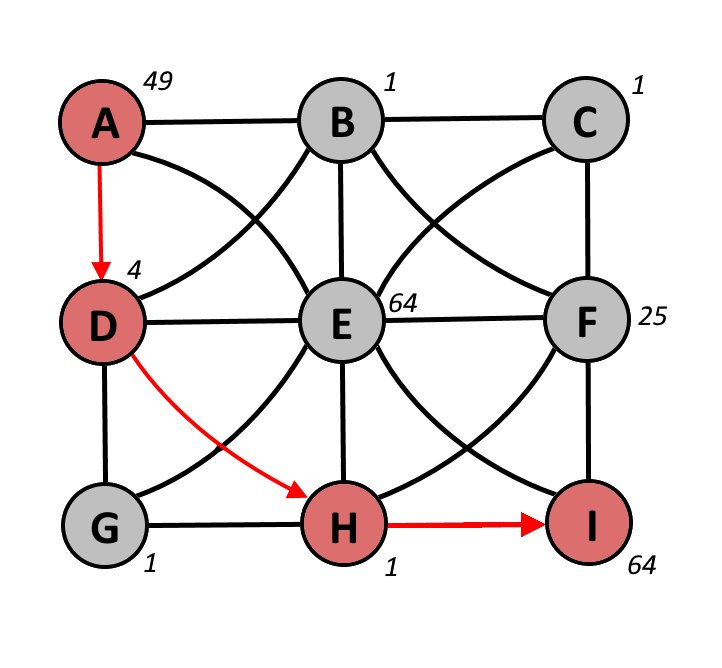
\includegraphics[scale=0.4]{Grafe.png}
\caption{Grafe met het kortste pad aangeduid}
\label{fig:Graph}
\end{figure}

\newpage
\section{Alternatieve Pixeldistance-formule}
We nemen nu een nieuwe afstandsfunctie $ \sqrt{r^2 + g^2} $ i.p.v. de originele functie $ \sqrt{r^2 + g^2 + b^2} $.

De blauwe component wordt nu dus niet meer bekeken bij het berekenen van de afstand tussen twee pixels. Hierdoor zal bijna iedere
afbeelding in de praktijk een snellere uitvoeringstijd kennen, omdat er minder berekeningen gebeuren. Hoe meer blauw er aanwezig is
in een afbeelding, of beter, hoe meer doorslaggevend blauw is voor de grens tussen twee afbeeldingen, hoe simpeler de grens er zal uitzien
als we de nieuwe afstandsfunctie gebruiken. De grens wordt dus versimpeld en de afbeelding zal er anders uitzien.

In een afbeeldingpaar zonder de kleur blauw zal deze nieuwe functie geen effect hebben op de grens. Anderzijds zal het programma geen goede grens vinden tussen
twee afbeeldingen waar enkel de kleur blauw in voorkomt. In dit geval zal het de korste weg in aantal pixels aanduiden als grens.
Dit komt omdat in zo'n afbeeldingenpaar de kost van een pixel altijd gelijk is aan 0, en dus is het gewicht van eenderwelk pad 0. Hierdoor gaat
het algoritme van Dijkstra zoeken naar een kortste pad in aantal pixels, omdat het stopt zodra het de eind-node heeft gevonden.

Het kan echter ook zijn dat dit pad zeer lang is. Dit hangt af van de implementatie van het algoritme. Omdat het gewicht van ieder pad gelijk
is aan 0, zal de PriorityQueue alle paden als \textquotedbl even lang\textquotedbl  zien, alhoewel dat niet altijd zo is. Zo kan het dus ook zijn dat een bepaald
(puur blauw) afbeeldingenpaar een zeer lange uitvoeringstijd heeft omdat de grens voortdurend heen en weer gaat.

\section{Tijdscomplexiteit}




\end{document}
